
\clearpage
\section{La fonction d'importation}

\begin{wrapfigure}[3]{l}{5.5cm}   % [x] Wie manche Zeile soll sich um die Grafik "brechen"
  \vspace{-35pt}      % Grundwert war 20; mit 30 schön oben beim Text ausgerichtet
  \begin{center}
    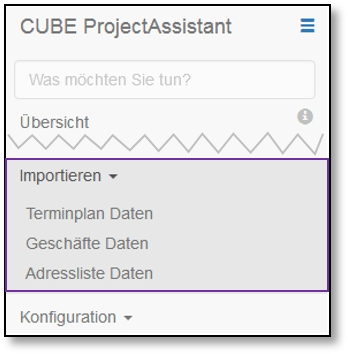
\includegraphics[width=1\linewidth]{../chapters/12_Importieren/pictures/12_Menu_Importieren.jpg}
  \end{center}
  \vspace{-20pt}
  \caption{Importer des données}
  \vspace{-10pt}
\end{wrapfigure}

Dans le menu à gauche, sélectionnez l'élément de menu 'Importer' et le sous-élément désiré : données d'échéanciers, de transactions ou de liste d'adresses.

\vspace{5.5cm}

\subsection{Données d'échéancier}
\label{bkm:Ref445411998}

\begin{wrapfigure}[10]{r}{6.5cm}
\vspace{-15pt}
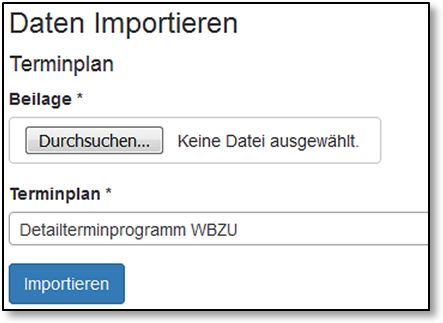
\includegraphics[height=50mm]{121_DatenImportieren.jpg}
\caption{Importer des données}
\end{wrapfigure}
La fonction d'importation 'Données d'échéancier' vous permet d'importer un nouvel échéancier détaillé et mis à jour. La planification du projet s'effectue dans Microsoft Project, est exportée en tant que fichier XML, et ensuite importée dans CUBE PA. Les données existantes dans CUBE PA sont ainsi remplacées. Les données importées ne peuvent pas être modifiées, elle peuvent uniquement être visualisées. Il est également possible de visualiser le planning du projet et d'agrandir la période désirée sur des ordinateurs sans Microsoft Project. Vous trouverez des informations plus détaillées à ce sujet dans le chapitre \ref{bkm:Ref445400921} 'Le planning'.

\vspace{\baselineskip}

Afin de pouvoir utiliser les options de visualisation et de filtrage (projet / sous-projet / ressources) dans CUBE PA, le fichier MS Project doit déjà contenir les informations correspondantes. Les ressources sont définies à l'avance selon les procédures usuelles de MS Project et sont ensuite attribuées aux processus individuels. L'attribution des processus à un projet / sous-projet se fait par le moyen de champs définis par l'utilisateur. A cet effet, deux nouvelles colonnes sont à ajouter dans le fichier MS Project (type texte, par exemple Texte1 et Texte2). Ces colonnes doivent être nommées 'Subproject\_1' et 'Subproject\_2' \col{(1)}, soit directement dans le tableau ou sous Format, Champs définis par l'utilisateur. Ceci permet de correctement importer les données dans CUBE PA. Les processus individuels peuvent ensuite être attribués aux projets (sous-projets) selon la définition des tags dans CUBE PA. Pour ce faire, les noms de projets peuvent être saisis manuellement ou par le moyen des menus déroulants dans les colonnes 'Subproject\_1' et 'Subproject\_2'. Avant d'exporter/importer, vérifiez que tous les processus sont attribués aux bons projets et qu'aucun champ n'est resté vide. C'est le seul moyen pour assurer que les processus ne soient pas masqués par erreur par le filtrage qui suivra dans CUBE PA.

\begin{figure}[H]
\center{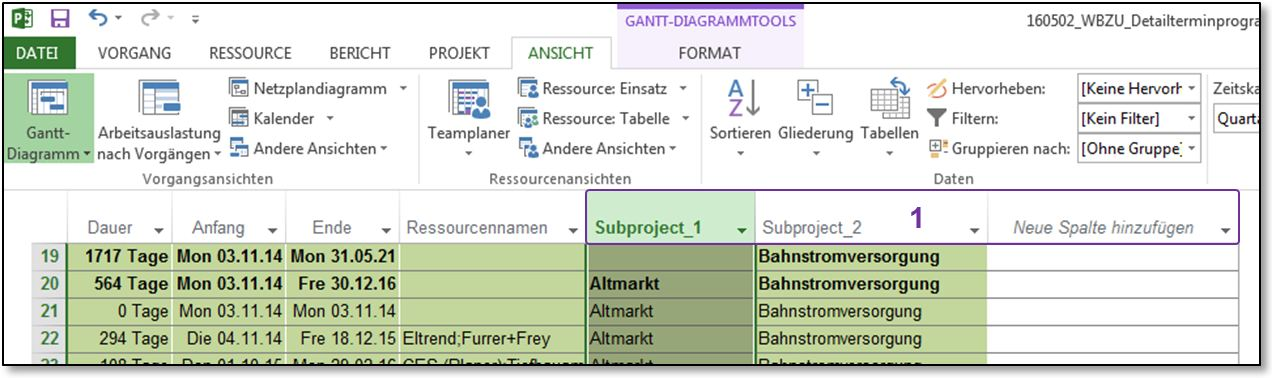
\includegraphics[width=1\linewidth]{121_zusSpaltenMSProject.jpg}}
\caption{Colonnes supplémentaires nécessaires dans MS-Project}
% \label{fig:speciation}
\end{figure}

\subsection{Données de transactions}

Ce chapitre suivra plus tard.

\subsection{Données de liste d'adresses}

Il est possible d'importer dans CUBE PA une liste d'adresses créée avec Excel ou en format Excel.

\begin{figure}[H]
\center{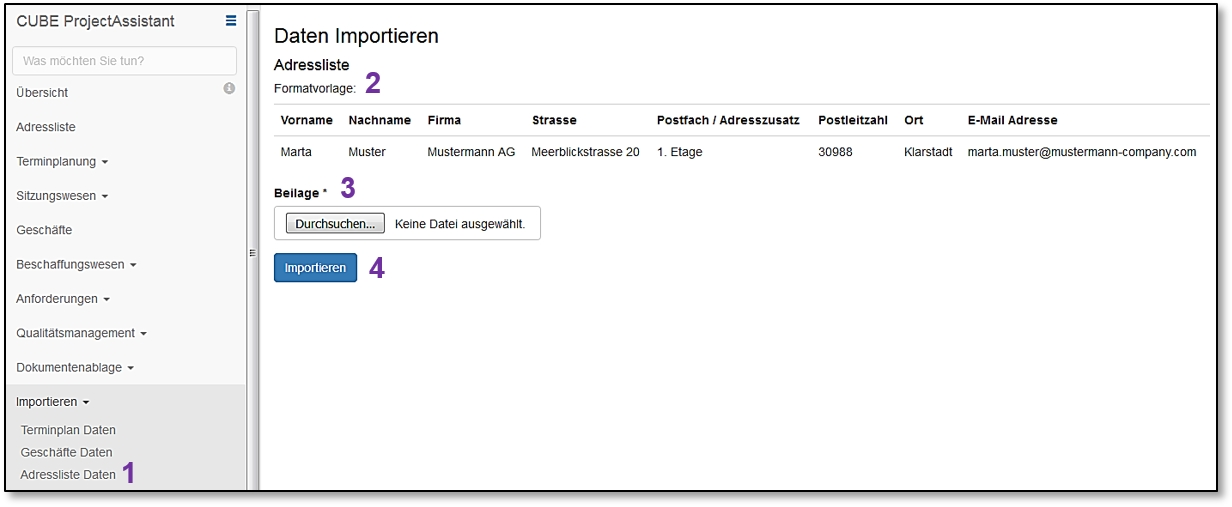
\includegraphics[width=1\linewidth]{../chapters/12_Importieren/pictures/12_Adressdaten_impUebersicht.jpg}}
\caption{Importer une liste d'adresses Excel}
% \label{fig:speciation}
\end{figure}

Dans le menu à gauche, cliquez sur l'élément de menu 'Importer' puis sur le sous-élément 'Données de liste d'adresses' \col{(1)}. Préparez le fichier Excel selon les colonnes nécessaires indiquées sous 'Format' \col{(2)} afin de garantir le succès de l'importation des données.

\vspace{\baselineskip}

Cliquez sur 'Parcourir' \col{(3)} et choisissez ensuite le document désiré dans la fenêtre Explorer. Après avoir choisi le fichier Excel, cliquez sur 'OK' et vous pouvez ensuite vérifier quel fichier sera importé :

\begin{figure}[H]
\center{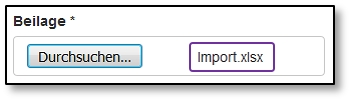
\includegraphics[width=.5\linewidth]{../chapters/12_Importieren/pictures/12_Listenimport.jpg}}
\caption{Choisir un fichier}
% \label{fig:speciation}
\end{figure}

Si tout est correct, cliquez sur le bouton 'Importer' \col{(4)}. Les adresses seront importées et seront ensuite disponibles dans le menu 'Liste d'adresses'.

\vspace{\baselineskip}

Suite à l'importation, une liste des adresses qui ont été importées est affichée. Vous pouvez ainsi vérifier si l'importation s'est déroulée correctement :

\begin{figure}[H]
\center{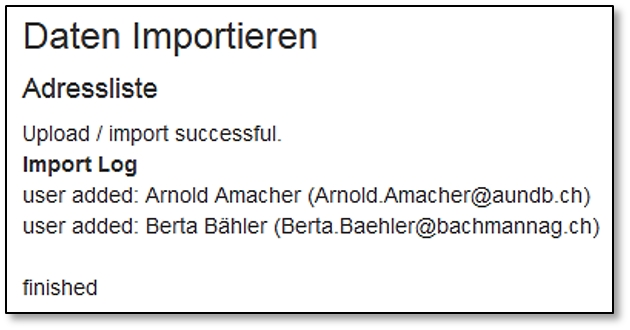
\includegraphics[width=.5\linewidth]{../chapters/12_Importieren/pictures/12_Import_ok.jpg}}
\caption{Procès-verbal d'importation}
% \label{fig:speciation}
\end{figure}

En cas de problème lors de l'importation, un message d'erreur apparaît.